\documentclass[9pt,a5paper]{extarticle}
\usepackage[margin=.7cm]{geometry}
\usepackage[utf8]{inputenc}
\usepackage[IL2]{fontenc}
\usepackage[czech]{babel}
\usepackage{microtype}
\usepackage{amssymb}
\usepackage{amsthm}
\usepackage{amsmath}
\usepackage{xcolor}
\usepackage{graphicx}
\usepackage{wasysym}
\usepackage{multicol}

\usepackage[inline]{enumitem}

\newcommand{\R}{\mathbb{R}}

\newcommand{\hint}[1]{{\color{gray}\footnotesize\noindent(Nápověda: #1)}}

\setlist[enumerate]{label={(\alph*)},topsep=\smallskipamount,itemsep=\smallskipamount,parsep=0pt,itemjoin={\quad},leftmargin=1cm}
\setlist[itemize]{topsep=\smallskipamount,noitemsep}

\def\tisk{%
\newbox\shipouthackbox
\pdfpagewidth=2\pdfpagewidth
\let\oldshipout=\shipout
\def\shipout{\afterassignment\zdvojtmp \setbox\shipouthackbox=}%
\def\zdvojtmp{\aftergroup\zdvoj}%
\def\zdvoj{%
    \oldshipout\vbox{\hbox{%
        \copy\shipouthackbox
        \hskip\dimexpr .5\pdfpagewidth-\wd\shipouthackbox\relax
        \box\shipouthackbox
    }}%
}}%

\let\results\newpage
\let\endresults\relax

\def\resultssame{%
    \long\def\results##1\endresults{%
        \vfill
        \noindent\rotatebox{180}{\vbox{##1}}%
    }%
}


\newtheorem*{poz}{Pozorování}

\theoremstyle{definition}
\newtheorem{uloha}{\atr Úloha}
\newtheorem{suloha}[uloha]{\llap{$\star$ }Úloha}
\newtheorem*{bonus}{Bonus}
\newtheorem*{defn}{Definice}

\pagestyle{empty}

\let\ee\expandafter

\def\vysld{}
\let\printvysl\relax

\makeatletter
\long\def\vyslplain#1{\ee\ee\ee\gdef\ee\ee\ee\vysld\ee\ee\ee{\ee\vysld\ee\printvysl\ee{\the\c@uloha}{#1}}}
\let\vysl\vyslplain

\def\locvysl#1{\ee\gdef\ee\locvysld\ee{\locvysld\item #1}}
\let\lv\locvysl

\newenvironment{ulohav}[1][]{\begin{uloha}[#1]\gdef\locvysld{\begin{enumerate*}}}{\ee\vyslplain\ee{\locvysld\end{enumerate*}}\end{uloha}}
\def\stitem{\@noitemargtrue\@item[$\star$ \@itemlabel]}
\def\ststitem{\@noitemargtrue\@item[$\star\star$ \@itemlabel]}

\makeatother

\def\atr{}
\def\basic{\def\atr{\llap{\mdseries$\sun$ }\gdef\atr{}}}
\def\interest{\def\atr{\llap{$\star$ }\gdef\atr{}}}
\def\iinterest{\def\atr{\llap{$\star\star$ }\gdef\atr{}}}
\let\mb\mathbf

\begin{document}

% \tisk
%\resultssame

\section*{25. Důkazní materiál}


\begin{uloha} % https://matheducators.stackexchange.com/a/11840
Zde jsou \emph{axiomy} naší oblíbené \uv{student-seminářové} situace:
\begin{enumerate}[label={(A\arabic*)}]
    \item Na každé přímce leží jiná kolekce bodů. (Neboli: Přímka \emph{je} kolekce bodů.)
    \item Existují alespoň dva body.
    \item Každé dva různé body leží na právě jedné společné přímce.
    \item Pro každou přímku existuje bod, který na ní neleží.
    \item Jestliže na přímce $p$ neleží bod $A$, pak existuje právě jeden přímka rovnoběžná s $p$, na které $A$ leží.\label{rovnobeznost}
\end{enumerate}
Navíc jsme již dokázali tyto \emph{věty}:
\begin{enumerate}[label={(V\arabic*)}]
    \item Každý bod leží na alespoň dvou přímkách.\label{dve-primky}
    \item Na každé přímce leží alespoň jeden bod.\label{aspon-jeden}
\end{enumerate}
Dokažte následující tvrzení:
\begin{enumerate}[resume,label={(V\arabic*)}]
    \item Na každé přímce leží alespoň dva body. \hint{Postupujte sporem, již víme z \ref{aspon-jeden}, že tam aspoň jeden bod leží, ten podle \ref{dve-primky} leží ještě na nějaké další přímce. Směřujte ke sporu s \ref{rovnobeznost} pomocí toho, že obě tyto přímky budou rovnoběžky k nějaké třetí.} \label{aspon-dva}
    \item Existují alespoň čtyři body. \hint{První tři získáte snadno z axiomů, čtvrtý bod pak z \ref{aspon-dva} a \ref{rovnobeznost}.}\label{ctyri-body}
    \item Existuje alespoň šest přímek. \hint{Začněte jako v důkazu \ref{ctyri-body} a ukažte, že každá dvojice bodů leží na jiné přímce.}
    \ststitem Na každé přímce leží stejný počet bodů (aspoň pokud je celkové množství bodů konečné.)
\end{enumerate}
\end{uloha}

\interest
\begin{uloha}
Zkonstruujte situaci (tzv. \emph{model}) splňující axiomy z předchozí úlohy, který bude obsahovat právě $9$ bodů. \hint{Uspořádejte si je do čtverce a dělejte \uv{něco jako přímky}.}
\end{uloha}


\begin{uloha}
Nalezněte chybu v tomto důkazu $1=2$: Předpokládejme, že $1 = 2$, pak ze symetrie rovněž platí $2 = 1$. Součtem těchto dvou rovností dostaneme $3 = 3$, což je pravda, tudíž tvrzení platí.
\end{uloha}


\begin{uloha}
Nalezněte chybu v tomto důkazu $1=2$: Nechť jsou $a$, $b$ nenulová reálná čísla, která se rovnají. Upravujme:
\begin{align*}
    a&=b \\
    a^2 &= ab \\
    a^2 - b^2 &= ab - b^2 \\
    (a+b)(a-b) &= b(a-b) \\
    a+b &= b \\
    2b &= b\ (\text{protože }a=b) \\
    2 &= 1
\end{align*}
\end{uloha}


\begin{uloha}[Pro znalce integrálního počtu]
\def\dx{\,\mathrm{d}x}
Nalezněte chybu v tomto důkazu $0=1$:
\[ \int \frac1x \dx = \int 1 \cdot \frac1x \dx \stackrel{\substack{\text{per}\\ \text{partes}}}= x \cdot \frac1x - \int x \cdot \left(-\frac1{x^2}\right) \dx = 1 + \int \frac1x \dx, \]
tudíž $0 = 1$.
\end{uloha}

\basic
\begin{uloha}[Anglický vtip; oceníte?]
Proof that a dog has 9 legs:
\begin{itemize}
    \item No dog has 5 legs.
    \item A dog has 4 more legs than no dog.
    \item Therefore, a dog has 9 legs.
\end{itemize}

\end{uloha}



% \begin{ulohav}
% Nalezněte rovnice všechny tečen ke křivce $K$ procházející bodem $B$:
% \begin{enumerate}
%     \item $\frac{x^2}{25} + \frac{y^2}{100} = 1$, $B[1;14]$\lv{$y = \frac32 x + \frac{25}{2}$ a $y = -\frac83 x - \frac{50}{3}$ (body dotyku $[-3;8]$ a $[4;6]$)}
%     \item $(x+1)^2 + (y+1)^2 = 4$, $B[13;7]$\lv{$y=\frac{5}{12}x + \frac{9}{12}$a $y=\frac{3}{4}x-\frac{11}{4}$ (body dotyku $[]$)}
% \end{enumerate}
% \end{ulohav}


%\begin{uloha}
%Napište rovnice všech možných hyperbol, jejichž osy splývají s osami souřadnic a které prochází body $K[2;1]$ a $L[8;-2]$.\vysl{$-\frac{x^2}{16} + \frac{y^2}{\frac45} = 1$}
%\end{uloha}
%
%\begin{ulohav}
%Pro hyperbolu $h$ danou rovnicí $x^2 - y^2 = 1$ nalezněte všechny přímky rovnoběžné s~přímkou $p$, které budou mít s $h$ právě jeden společný bod, jestliže $p$ je
%\begin{enumerate*}
    %\item $x = 0$,\lv{$x = \pm 1$}
    %\item $y = 0$,\lv{žádná neexistuje}
    %\item $y = 2x$,\lv{$y = 2x \pm \sqrt3$}
    %\item $y = x$,\lv{$y = x + c$, kde $c \in \R \setminus\{0\}$}
%\end{enumerate*}
%\end{ulohav}


%\[ 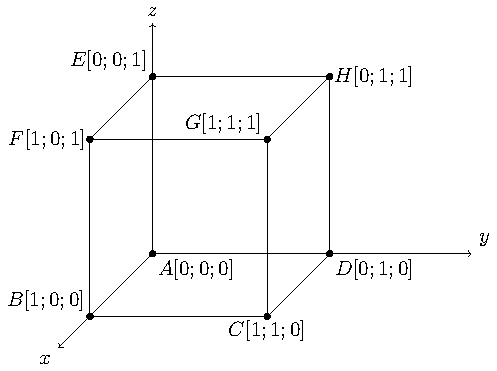
\includegraphics{krychle_std.pdf} \]
%\emph{Všechny úlohy se postupně odkazují na tytéž body, přímky atd.}



%\renewcommand{\baselinestretch}{1.25}
\baselineskip=1.25\baselineskip
\setlist[enumerate]{label=\textbf{(\alph*)},itemjoin={\quad}}

\results
\parindent=0pt
% \parskip=\smallskipamount
\rightskip=0pt plus1fil\relax
\def\printvysl#1#2{\textbf{#1.} #2\par}
\def\printalphvysl#1#2#3{\textbf{#1}(#2)\ #3\par}
\vysld
\endresults
%}

%\copy0
%
%\vfil
%
%\box0
%\eject
\unvbox0



\end{document}
